\documentclass{article}

\usepackage{color}
\usepackage{listings}
\usepackage{graphicx}
\usepackage{subfig}

\definecolor{MyYellow}{rgb}{1,1,0.8}

\lstset{language=Matlab,backgroundcolor=\color{MyYellow},basicstyle=\footnotesize,numberstyle=\footnotesize,numbers=left,stepnumber=1,numbersep=5pt,breaklines=true,frame=lines,tabsize=2}

\author{Ruurd Moelker \and Jan Paul Posma}
\date{\today}
\title{Signalen \& Systemen \\Practicum 3}

\begin{document}
\maketitle

\section{Opgave 1}
Om de convolutie in matlab te bepalen gebruiken wij het commando:
$conv(xx,~[1,~-0.9])$
De filterco\"efici\"enten zijn hierbij 1 en 0.9.

Het invoersignaal $x[n]$ is de reeks van getallen startende met 10 maal 256 gevolgd door 40 maal een 0 waarna de reeks zich herhaald tot 101 getallen zijn bereikt.

\section{Opgave 2}
De stemplot van $x[n]$ in te zien samen met de stemplot van $w[n]$ in figuur \ref{fig_opgave2}. Het signaal $x[n]$ is omschreven in de vorige opgave. $w[n]$ heeft deze vorm omdat het filter als het ware het effect heeft van de afgeleiden berekenen gemixed met een verzwakking van het signaal met een factor 0.1. Bij de wisseling tussen hoog en laag in $x[n]$ heeft $w[n]$ een piek danwel dal. De pieken zijn 256 hoog omdat deze voorafgaan in $x[n]$ door nullen. De dalen daarentegen zijn niet -256 diep, omdat deze verwoven is met nog 10\% van het signaal $x[n-1]$. Tussen top en dal zit een gebied in $w[n]$ met waarde 10\% van $x[n]$.

\begin{figure}[h]
  \centering
 	\subfloat[][signal x]{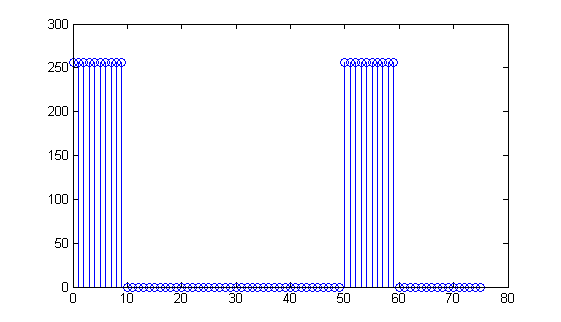
\includegraphics[width=0.4\textwidth]{content/2xx.png}}
	\subfloat[][signal w]{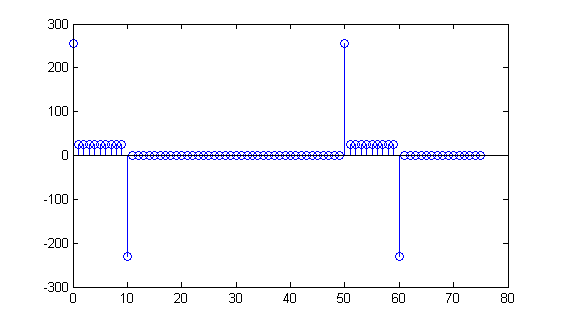
\includegraphics[width=0.4\textwidth]{content/2ww.png}}
  \caption{Stemplot van x en w over het interval [0..75]}
  \label{fig_opgave2}
\end{figure}

\section{Opgave 3}
Het matlab commando $length()$ geeft de lengte van een signaal. Voor $x[n]$ is deze lengte 101 en voor $w[n]$ is de lengte 102. De lengte van de convolutie wordt bepaald door $length(xx)+length(bb)-1$ waarbij bb de vector met co\"efficienten is, in dit geval [1, -0.9], dus lengte 2. Tezamen geeft dit $w[n]$ de lengte:  $101+2-1 = 102$.

\section{Opgave 4}
Restauratie van het orginele signaal $x[n]$ uit $w[n]$ kan met behulp van de matlab functie: 
$$yy = conv(ww, rr)$$
\begin{center}
waarbij\\
$r = 0.9$, $M = 22$ en $rr = r .^ (0:M)$
\end{center}


\section{Opgave 5}
In figuur \ref{opgave5} is de benadering van $x[n]$ door de convolutie van de reeks $rr$ op $w[n]$ geplot in een stem grafiek.
\begin{figure}[h]
  \centering
 	\subfloat[][signaal w]{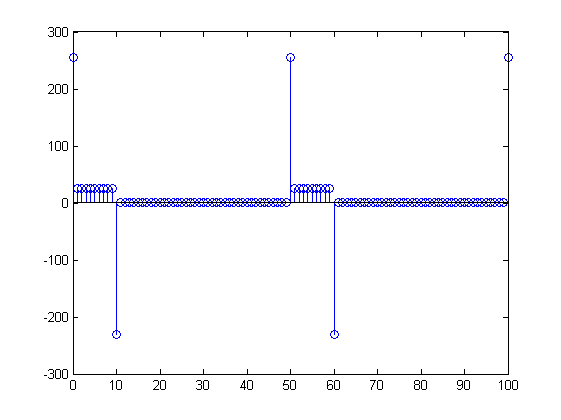
\includegraphics[width=0.4\textwidth]{content/5ww.png}}
	\subfloat[][signaal y]{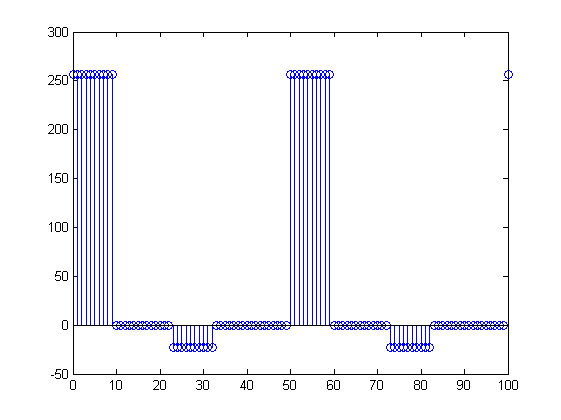
\includegraphics[width=0.4\textwidth]{content/5yy.png}}
  \caption{Stemplot van w en de benadering van w van x}
  \label{opgave5}
\end{figure}
\newpage
\section{Opgave 6}
In figuur \ref{opgave6} is het verschil tussen het oorspronkelijke signaal x, uitgezet tegen het herstelde signaal y. Het figuur laat zien dat het herstelde signaal erg goed overeenkomt omdat het verschil bijna overal 0 is. Echter is tussen n = 23 en n = 33 het verschil ineens een maximale grote van 23. Dit komt omdat vanaf dat punt de piek in het tussen signaal w niet meer binnen het bereik is van de restauratiefilter.

\begin{figure}[h]
  \centering
 	\subfloat[][signaal x]{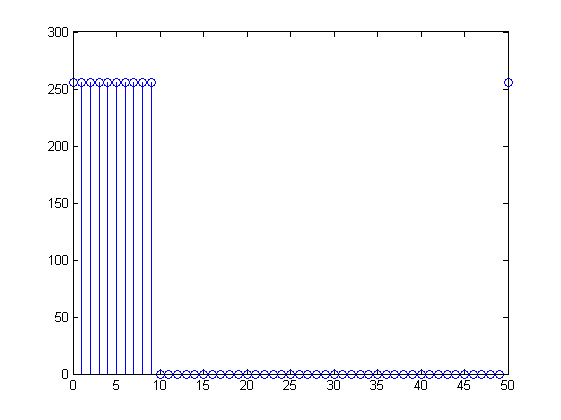
\includegraphics[width=0.4\textwidth]{content/6xx.png}}
	\subfloat[][signaal y]{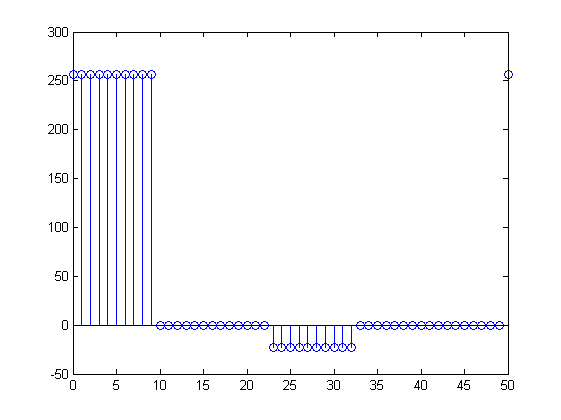
\includegraphics[width=0.4\textwidth]{content/6yy.png}}
	\subfloat[][signaal x - signaal y]{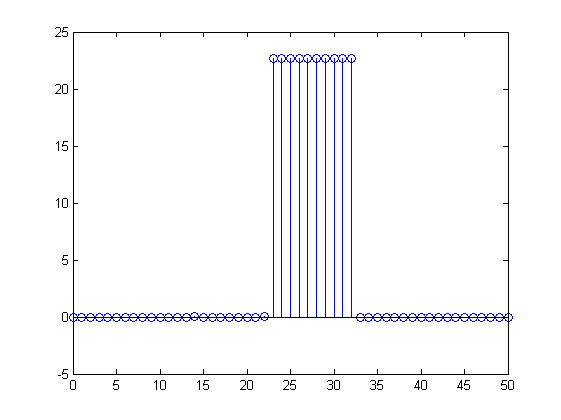
\includegraphics[width=0.4\textwidth]{content/6.png}}
  \caption{stemplot verschil signalen x en y over het interval [0..50]}
  \label{opgave6}
\end{figure}

\section{Opgave 7}
De waarde van r wordt bepaald door de sterkte die we aan de echo toekennen, het is immers de amplitude van het signaal P tijdeenheden terug dus. Omdat de echo 90\% van het oorspronkelijke signaal moet zijn geldt $r = 0.9$. P is de tijdverschuiving van de echo uitgedrukt in tijdseenheden van de sample frequentie dus $p = \delta~t*f_s = 8000 * 0.2 = 1600$.

\newpage
\section{Opgave 8}
De echo van een signaal kan met een FIR filter gemaakt worden waarbij de reeks van filterco\"efici\"enten bestaan uit een \'e\'en gevolgd door een reeks nullen, eindigend op de waarde van r. Preciezer zij de filterco\"efici\"enten als volgt: $[1, 0_1, 0_2, .. 0_{p-1}, 0.9]$. In matlab wordt het nieuwe signaal yy uit bronsignaal x2 berekend door middel van: $yy = conv(x2, [1 zeros(1,8000*0.2 - 1) 0.9]);$. 

Het oorspronkelijke signaal x2 en gefilterd signaal yy zijn uitgezet in figuur \ref{fig:opgave8}.

%
%
% UITLEG FIGUUR NOG NODIG!!!!!!!!!!!!!!!!!!!!
%
%

\begin{figure}[h]
  \centering
 	\subfloat[][x2]{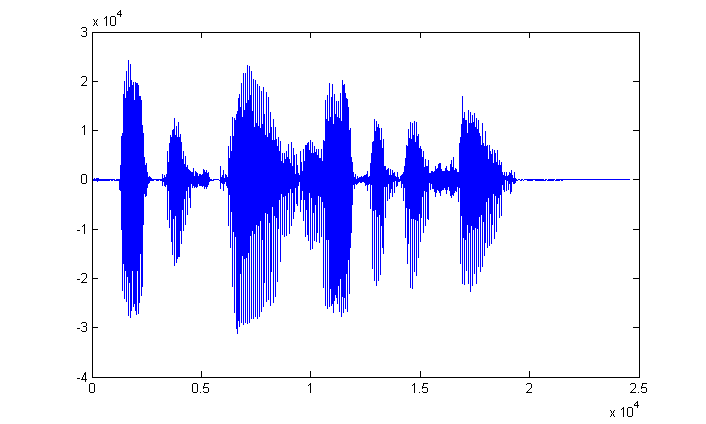
\includegraphics[width=0.4\textwidth]{content/8x2.png}}
	\subfloat[][yy]{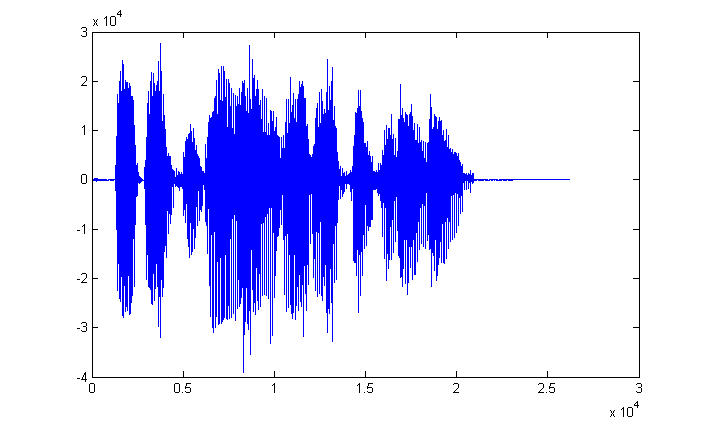
\includegraphics[width=0.4\textwidth]{content/8yy.png}}
  \caption{Het orginele signaal x2 verkregen uit functie labdat.mat en het signaal met echo yy}
  \label{fig:opgave8}
\end{figure}

\end{document} 